%%%%%%%%%%%%%%%%%%%%%%%%%%%%%%%%%%%%%%%%%%%%%%%%%%%%%%%%%%%%%%%%%%%%%%%%%%%%%%%%%%%%%%%%%%%%%%%%%%%%%%%
%%%%%%%%%%%%%% Template de Artigo Adaptado para Trabalho de Diplomação do ICEI %%%%%%%%%%%%%%%%%%%%%%%%
%% codificação UTF-8 - Abntex - Latex -  							     %%
%% Autor:    Fábio Leandro Rodrigues Cordeiro  (fabioleandro@pucminas.br)                            %% 
%% Co-autor: Prof. João Paulo Domingos Silva  e Harison da Silva                                     %%
%% Revisores normas NBR (Padrão PUC Minas): Helenice Rego Cunha e Prof. Theldo Cruz                  %%
%% Versão: 1.0     13 de março 2014                                                                  %%
%%%%%%%%%%%%%%%%%%%%%%%%%%%%%%%%%%%%%%%%%%%%%%%%%%%%%%%%%%%%%%%%%%%%%%%%%%%%%%%%%%%%%%%%%%%%%%%%%%%%%%%
\section{\esp Introdução}

Um grafo conexo e sem articulações é chamado 2-conexo (ou biconexo) e é amplamente utilizado no contexto da área da computação pois apresenta propriedades interessantes, tal como definir um grafo como “tolerante a falhas”. Denominam-se componentes biconexos de um grafo G aos subgrafos maximais de G que sejam biconexos em vértices, ou isomorfos a K2. Cada componente biconexo é também chamado de bloco do grafo. Assim se G é biconexo então ele possui um único bloco, que coincide com o próprio G. 


O problema consiste em encontrar o conjunto K de componentes biconexos, ou blocos, utilizando três abordagens que consistem em localizar os mesmos utilizando ciclos, articulações ou um método já pronto.


Neste trabalho estaremos explorando essas possíveis soluções para esse problema. No intuito de testar e avaliar o desempenho dos nossos algoritmos utilizaremos instâncias geradas por um algoritmo de geração de grafos conexos pseudoaleatórios que garante articulações e pontes.

\section{\esp {Implementação}}

Para o desenvolvimento dos algoritimos estudados neste trabalho, foi escolhia a linguagem C++ por ser uma linguagem multiparadigma e de alta performance. 
Foi feito uma classe para manter a estrutura de dados do grafo, no qual foi representado utilizando uma lista de adjacência, bem como os métodos de identificação de blocos e de geração aleatória de grafos, desenvolvidos para serem executados de forma sequencial.

\subsection{\esp Estrutura de Dados}

Foi definido previamente que os grafos analisados deveriam ser simples não direcionados e conexos além de que as arestas não necessitavam de informações adicionais, sendo assim foi escolhido a lista de adjacência como forma de representação do grafo, por consumir menos espaço em memória que a matriz de adjacência e maior flexibilidade.

\subsection{\esp Algoritmos}

Foram utilizados algoritmos importantes para o objetivo do estudo, como métodos que verificam a existência de dois caminhos internamente disjuntos entre cada par de vértices, bem como um método que identifica articulações testando a conectividade após a remoção de cada vértice e o método proposto por Tarjan \cite{artigo_tarjan}.

\subsubsection{\esp Geração de Grafos}

Para possibilitar os testes e análises dos algoritimos de identificação de blocos, primeiramente foi necessário desenvolver um algoritmo de geração aleatória de grafos, que provesse customização de propriedades como número de vértices, densidade de arestas e probabilidade de blocos.

O algoritimo de geração de grafos desenvolvido (utilizado através de um construtor da classe) recebe como parâmetros o numero de vértices, o número de subgrafos iniciais (estes serão utilizados para gerar blocos) e a porcentagem desejada de desidade de arestas em cada um dos subgrafos inicias. O método então define tamanhos aleatórios para cada subgrafo inicial, constroi uma árvore geradora através dos vétices selecionados (para assegurar conectividade), adiciona novas arestas aleatóriamente (quantidade tende a densidade especificada) e então conecta os subgrafos, assim garantindo a presença de blocos no grafo final.

\subsubsection{\esp Método I - Existência de ciclos entre pares de vértices}
\label{method_I}
O primeiro algoritimo desenvolvido pode ser considerado a maneira mais intuitiva, dentre os demais, de se solucionar o problema de identificação de componentes biconexos. Ele se baseia em verificar a biconectividade de cada par de vértices por iteração sendo que esta verificação se baseia em fazer uma travessia baseada na busca em profundidade, porém esta revisita vértices a fim de achar todos os caminhos possíveis da fonte ao terminal, e então descarta aqueles que não são disjuntos.

Embora intuitivo é notavel que esta solução não é ótima visto que, a mesma realiza travessias redundantes para encontrar pares de vértices que já estavam presentes em soluções de caminhos disjuntos encontrados anteriormente.

\subsubsection{\esp Método II - Idêntificação de articulações por remoção de vértices}

O segundo algoritimo desenvolvido se baseia no fato de que os vértices ditos articulações são aqueles que delimitam a estensão do bloco, com isso ao identificar quais vértices são articulações é possível reduzir a quantidade de verificações de biconectividade entre vértices que deveriam ser feitas, uma vez que durante uma travessia ao encontrar uma articulação não e preciso continuar a travessia de tal caminho. 
O método primeiramente faz o descobrimento de articulações através da remoção de cada vértice, em seguida é feito uma busca no grafo resultante para verificar se parte dele está desconexa levando a identificar o vértice removido como uma articulação. Após a identificação de todas as articulações do grafo é possivel otimizar a verificação de biconectividade utilizando apenas as articulações como raízes de buscas em profundidade de modo a encontrar ciclos que identifiquem os demais vértices integrantes do bloco.
A solução desenvolvida no segundo método apesar de superior ao método anterior, também não é ótima pois é possivel perceber que a identificação de articulações por remoção é um passo custoso, que necessita ser feito a priori, além de que a identificação dos blocos ainda possui algumas travessias de caminhos redundantes.

\subsubsection{\esp Método III - Algoritimo de Tarjan adaptado para componentes biconexos}

O algoritmo de Tarjan é uma técnica de busca em grafos para encontrar componentes fortemente conexos. Ele foi desenvolvido pelo matemático americano Robert Tarjan em 1972 e é amplamente utilizado em diversas aplicações, desde algoritmos de análise de redes sociais até otimização de rotas em mapas.

O algoritmo é baseado em uma abordagem de busca em profundidadez, que atribui um número de ordem a cada vértice visitado e utiliza uma pilha para rastrear o caminho de volta. Com o uso dessa técnica, o algoritmo é capaz de identificar componentes fortemente conexos em tempo linear, tornando-o extremamente eficiente.

Para adaptar o algoritmo de Tarjan para encontrar componentes biconexos, foi necessário armazenar as arestas visitadas em uma pilha enquanto é realizada a busca em profundidade no grafo. Durante essa busca, o algoritmo também procura por pontos de articulação, que são vértices que, caso removidos do grafo, deixam o grafo desconexo ou aumentam o número de componentes fortemente conexos. Assim que um ponto de articulação é encontrado, todas as arestas visitadas durante a busca em profundidade a partir do vértice formam um componente biconexo. Quando a busca em profundidade é concluída para um componente conectado, todas as arestas presentes na pilha formam um componente biconexo. Caso não haja nenhum ponto de articulação no grafo, o grafo é biconexo e o próprio grafo é um componente biconexo. Com essa abordagem, o algoritmo de Tarjan pode ser utilizado para encontrar componentes biconexos em tempo linear.


\section{\esp Análise de Resultados}

A seguir será analisado os resultados de tempos obtidos por cada algoritmo em relação
a quantidade de vértices dos grafos. O testes foram todos executados na mesma máquina (AMD Ryzen™ 5 5600G @ 3.9GHz) e no mesmo compilador com os mesmos parâmetros de otimização (Clang 15.0.7 -O2). 
Foram geradas instâncias de grafos de 100, 1000, 10000 e 100000 vértices com densidades de arestas proximas de 20 a 80\%. Como já detalhado anteriormente, foram apenas utilizadas implementações de algoritimos sequências. Durante o planejamento dos testes definiu-se um limite superior de tempo (\textit{TIMEOUT}), de 30 minutos para execussão de cada algoritimo para cada instância.

Os resultados dos testes realizados estão graficamente representados na \textbf{Figura 1}.

Todos os dados obtidos pelos testes estão disponíveis na \textbf{Tabela 1}.

% Figura
\begin{figure}[ht]
	\centering	
	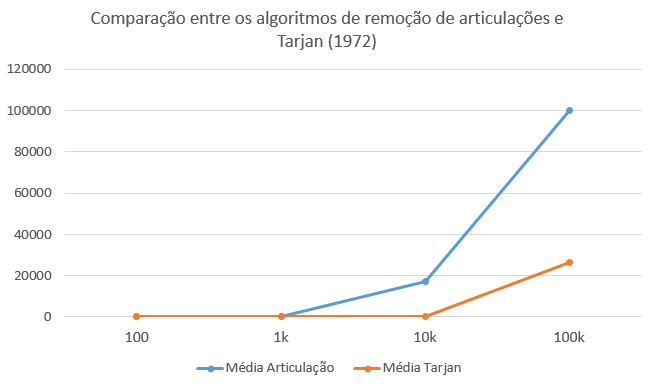
\includegraphics[scale=0.8]{figuras/sm_comparacao_art_tarj.png}
	% Caption centralizada
% 	\captionsetup{justification=centering}
     \vspace{-0.2cm}
	\\\textbf{\footnotesize Figura 1 - Comparação de algoritmos}
    \label{fig:figura1}
\end{figure}
\vspace{-0.5cm}

\subsection{\esp Análise Comparativa}

A imagem acima denota a ausência do método I (\ref{method_I}), visto que este obteve \textit{TIMEOUT} em todos as isntâncias do teste, porém foi-se verificado o funcionamento do algoritmo utilizando grafos manualmente elaborados (menos de 20 vértices). Acredita-se que a falta de testes completos pelo (\ref{method_I}) se dá por que este testa todos os caminhos possiveis entre cada par de vértices. 

Ao analisar o método de identificação de articulações, observou-se que ele apresentou tempos maiores em instâncias com menos arestas, isso se dá pois estes grafos tendem a possuir mais articulações, com isso necessitando de mais buscas.

Finalmente no algoritimo de Tarjan, este o único a completar a identificação dos blocos de todas as instâncias testadas, é visível a diferença em sua ordem de complexidade, linear no número de arestas, comparado as demais soluções toda via, ele se apresenta como um algoritimo bem menos intuitivo.

% Tabela
\begin{table}[htb]
	\centering
	\caption{\hspace{0.1cm} Tempos de execução}
	\vspace{-0.3cm} % espaço entre titulo e tabela
	\label{tab:tabela1}
	% Conteúdo da tabela
	\begin{tabular}{c|c|c|c|c}
  \hline
    \textbf{|V|} & \textbf{|E|} & \textbf{Caminhos Disjuntos} &  \textbf{Identificação de Articulação}	& \textbf{Tarjan (1972)}\\
    \hline
    100 & 250 & TIMEOUT & 907us & 52us \\
    100 & 600 & TIMEOUT & 412us & 121us \\
    100 & 800 & TIMEOUT & 490us & 132us \\
    1.000 & 3.000 & TIMEOUT & 95ms & 645us \\
    1.000 & 5.000 & TIMEOUT & 35ms & 1ms \\
    1.000 & 8.000 & TIMEOUT & 35ms & 2ms \\
    10.000 & 20.000 & TIMEOUT & 9s & 14ms \\
    10.000 & 50.000 & TIMEOUT & 31s & 89ms \\
    10.000 & 70.000 & TIMEOUT & 12s & 306ms \\
    100.000 & 200.000 & TIMEOUT & TIMEOUT & 3s \\
    100.000 & 400.000 & TIMEOUT & TIMEOUT & 13s \\
    100.000 & 800.000 & TIMEOUT & TIMEOUT & 63s \\ 
     \hline
 \end{tabular}
 	\vspace{.1cm}  %espaço entre tabela e fonte
	\small
	% Fonte
	{\footnotesize\\ \textbf{Fonte: Elaborado pelos Autores}}
\end{table}

\pagebreak

\section{\esp Conclusão}
Concluindo, este artigo apresentou a documentação do Trabalho Prático I, que teve como objetivo principal encontrar componentes biconexos de um grafo, ou seja, identificar blocos em grafos conexos com tamanhos variados de vértices e arestas.

Foram implementadas e comparadas três formas distintas para resolução do problema, sendo elas: o método que verifica a existência de dois caminhos internamente disjuntos (ou um ciclo) entre cada par de vértices do bloco, o método que identifica articulações testando a conectividade após a remoção de cada vértice, e a melhor solução que garante a resposta com uma boa complexidade, utilizando o método de Tarjan.

Os resultados obtidos indicaram que o método proposto por Tarjan apresentou a melhor performance em termos de tempo de execução e consumo de recursos, tornando-se uma solução eficiente para o problema em questão.

